\documentclass[11pt,a4paper]{report}
\usepackage{marvosym}

\assignment{2}
\group{1 (Moodle), 39 (INGInious)t}
\students{Victor Carballes Cordoba (NOMA : 34472100)}{Krystian Targonski (NOMA : 42942000)}

\begin{document}

\maketitle

Answer to the questions by adding text in the boxes. You may answer in either \textbf{French or English}. Do not modify anything else in the template.  The size of the boxes indicate the place you \textbf{can} use, but you \textbf{need not} use all of it (it is not an indication of any expected length of answer). \textbf{Be as concise as possible! A good short answer is better than a lot of nonsense!}
%\bigskip

\section{Exercises (5~pts)}

\textit{The following figure assigns a unique letter to each node, and a unique number to each branch. Use it to answer the following questions.}
\begin{center}
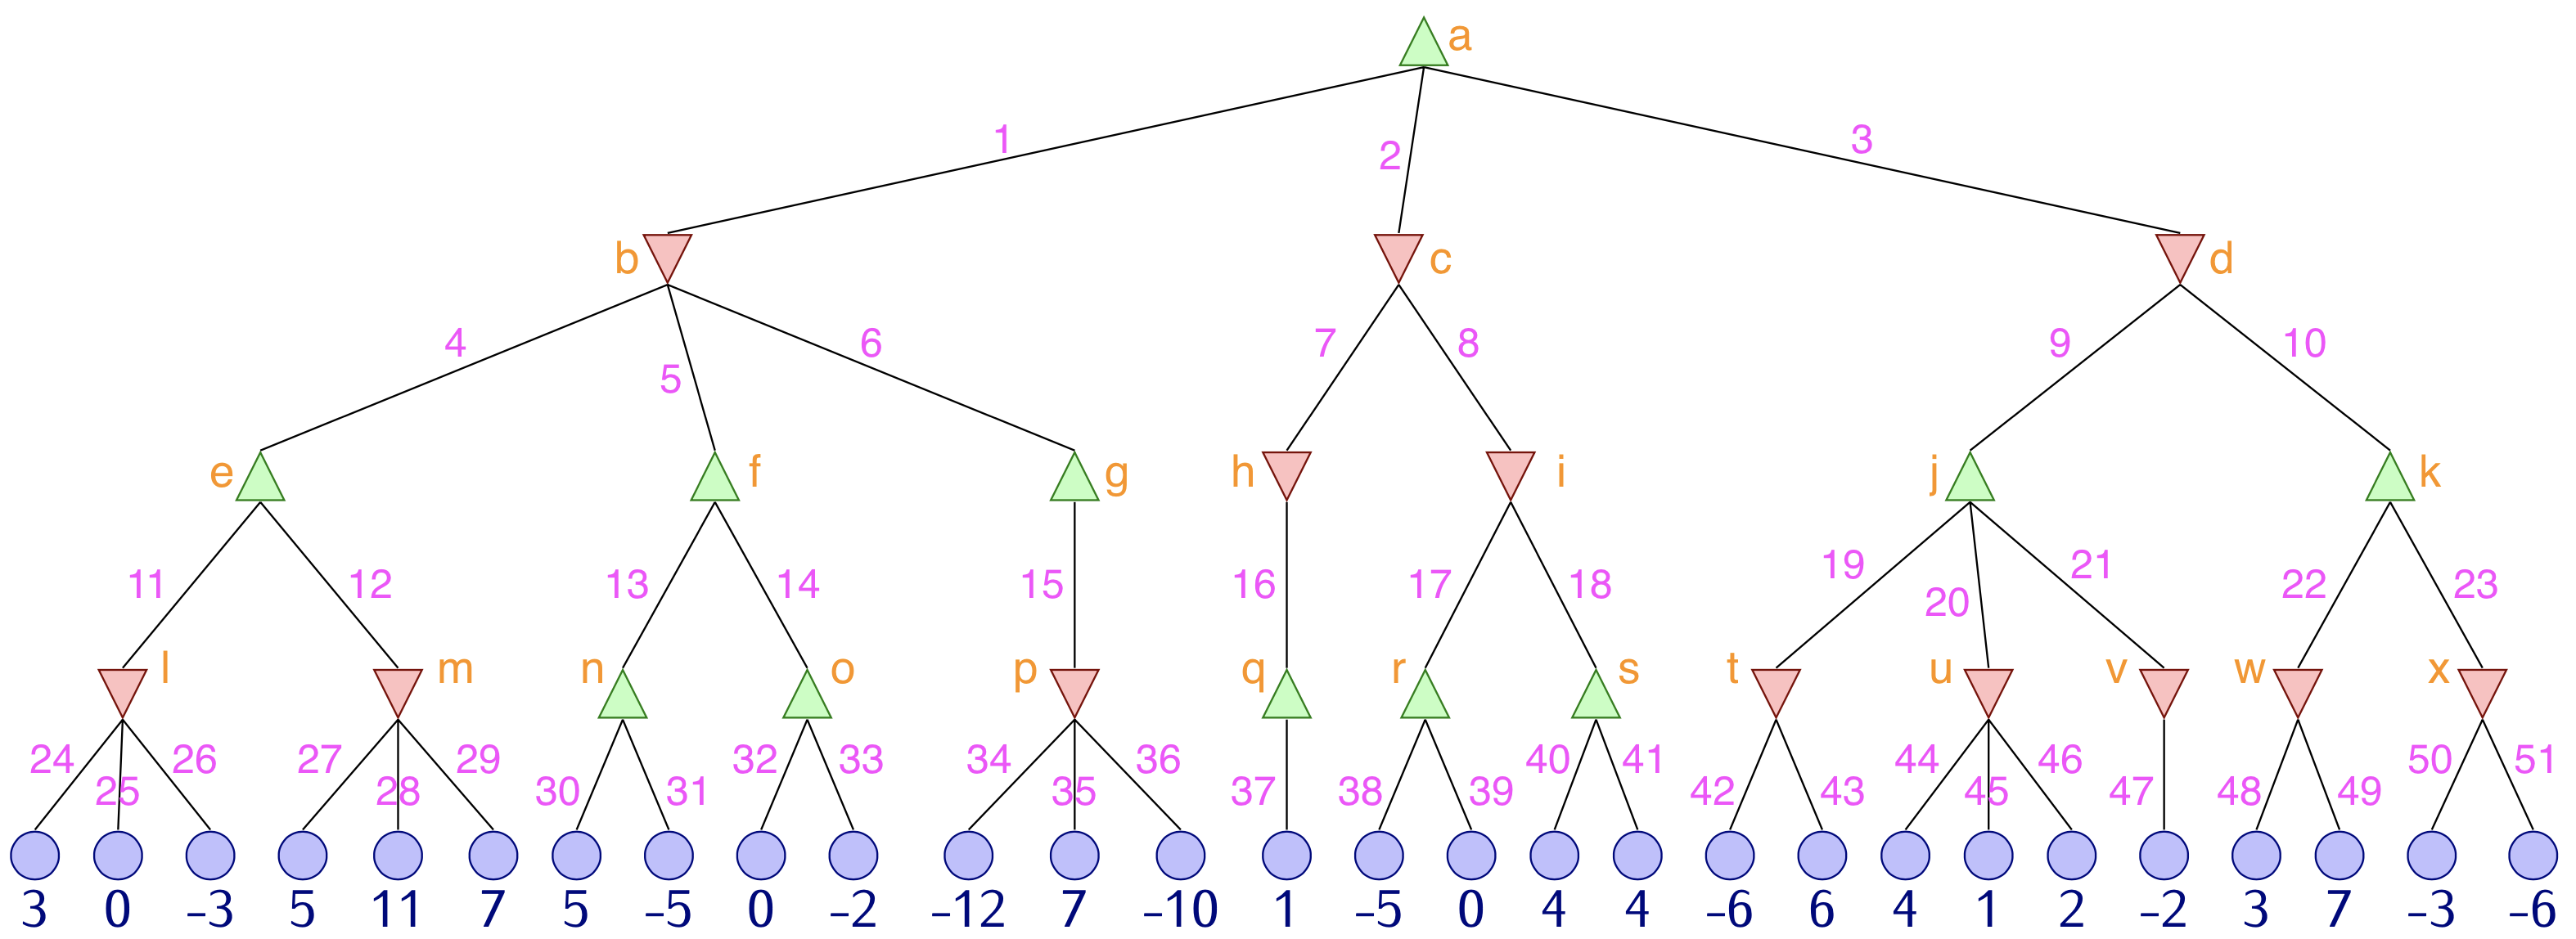
\includegraphics[width=\linewidth]{images/minimax_labelled.png}
\end{center}


\begin{enumerate}
\item Perform the MiniMax algorithm on the following tree, i.e.
      put a value to each node. What move should the root player do? \textbf{(1~pt)}
      
      \textit{Assign a numerical value to each node, and indicate the move (i.e.\! 1, 2, or 3) to perform:}
\end{enumerate}
    %TODO check
      \begin{answers}[3cm]
      \begin{multicols}{5}
      \textbf{a: 1} 

      \textbf{b: -12} 
      
      \textbf{c: 0} 
      
      \textbf{d: 1}
      
      \textbf{e: 5}
      
      \textbf{f: 5}
      
      \textbf{g: -12}
      
      \textbf{h: 1}
      
      \textbf{i: 0}
      
      \textbf{j: 1}
      
      \textbf{k: 3}
      
      \textbf{l: -3}
      
      \textbf{m: 5}
      
      \textbf{n: 5}
      
      \textbf{o: 0}
      
      \textbf{p: -12}
      
      \textbf{q: 1}
      
      \textbf{r: 0}
      
      \textbf{s: 4}
      
      \textbf{t: -6}
      
      \textbf{u: 1}
      
      \textbf{v: -2}
      
      \textbf{w: 3}
      
      \textbf{x: -6}
      
      \textbf{Move: 3}
      \end{multicols}
	  \end{answers}



\begin{enumerate}
\item[2.] Perform the Alpha-Beta algorithm on the same tree.
      At each non terminal node, put the successive values of $\alpha$ and
      $\beta$. Cross out the arcs reaching non visited nodes. Assume a
      left-to-right node expansion. \textbf{(1~pt)}
      
      \textit{Indicate the successive $\alpha$ and $\beta$ values of each node in the table below. Separate successive values by a comma (,). Indicate at the bottom the identifiers of the branches that are cut (in increasing order, separated by a comma) (indicate only the branches where the cuts happen, i.e.\!} don't \textit{indicate the branches that are below a cut).}
\end{enumerate}

\begin{answers}[8cm]
    %TODO check
    \begin{multicols}{2}
    \begin{tabular}{ccc}
    Node & $\alpha$ values & $\beta$ values\\
    \hline
    \textbf{a} &-inf,-12,0,1  &inf,1 \\ 
    \textbf{b} &-inf,-12  &inf,5,-12  \\
    \textbf{c} &-inf,0  &inf,1,0  \\
    \textbf{d} &-inf,1  &inf,1  \\
    \textbf{e} &-inf,-3,5 &inf,5  \\
    \textbf{f} &-inf,5  &inf  \\
    \textbf{g} &-inf,-12  &inf,-12  \\
    \textbf{h} &-inf,1  &inf,1  \\
    \textbf{i} &-inf,0  &inf,0  \\
    \textbf{j} &-inf,-6,1  &inf,1  \\
    \textbf{k} &-inf,3  &inf  \\
    \textbf{l} &-inf,-3  &3,0,-3  \\
    \textbf{m} &-inf,5  &5  \\ 
    \end{tabular}
    
    \begin{tabular}{ccc}
    Node & $\alpha$ values & $\beta$ values\\
    \hline
    \textbf{n} &5  &inf,5  \\
    \textbf{o} &/  &/  \\
    \textbf{p} &-inf,12  &-12  \\
    \textbf{q} &1  &1  \\
    \textbf{r} &-5,0  &inf,0  \\
    \textbf{s} &4  &inf,4  \\
    \textbf{t} &-inf,-6  &-6  \\
    \textbf{u} &-inf,1  &4,1  \\
    \textbf{v} &-2  &-2  \\
    \textbf{w} &-inf,3  &3  \\
    \textbf{x} &/  &/  \\
     &  &  \\
    \end{tabular}
    \end{multicols}
    
\textbf{Cuts: 14, 51} 
\end{answers}



\begin{enumerate}
\item[3.] Do the same, assuming a right-to-left node expansion instead.  \textbf{(1~pt)}
\end{enumerate}

\begin{answers}[8cm]
    %TODO check
      \begin{multicols}{2}
      \begin{tabular}{ccc}
      Node & $\alpha$ values & $\beta$ values\\
      \hline
      \textbf{a} &-inf,1 &inf \\ 
      \textbf{b} &-inf  &inf,-12  \\
      \textbf{c} &-inf  &inf,0  \\
      \textbf{d} &-inf,1  &inf,3,1  \\
      \textbf{e} &/  &/  \\
      \textbf{f} &/  &/  \\
      \textbf{g} &-inf,-12  &inf,-12  \\
      \textbf{h} &/  &/  \\
      \textbf{i} &-inf,0  &inf,4,0  \\
      \textbf{j} &-inf,-2,1  &inf,1  \\
      \textbf{k} &-inf,-6,3  &inf,3  \\
      \textbf{l} &/  &/  \\
      \textbf{m} &/  &/  \\ 
      \end{tabular}
      
      \begin{tabular}{ccc}
      Node & $\alpha$ values & $\beta$ values\\
      \hline
      \textbf{n} &/  &/  \\
      \textbf{o} &/  &/  \\
      \textbf{p} &-inf,-12  &-10,-12  \\
      \textbf{q} &/  &/  \\
      \textbf{r} &0  &inf,0  \\
      \textbf{s} &4  &inf,4  \\
      \textbf{t} &-inf,-6  &6,-6  \\
      \textbf{u} &-inf,1  &2,1  \\
      \textbf{v} &-2  &-2  \\
      \textbf{w} &-inf,3  &7,3  \\
      \textbf{x} &-inf,-6  &-6  \\
       &  &  \\
      \end{tabular}
      \end{multicols}
      
\textbf{Cuts: 4, 5, 7} 
\end{answers}




\clearpage
\begin{enumerate}
    \item[4.] Is there a node ordering that can lead to a more optimal pruning of the tree
(in the sense where the algorithm prunes more branches than in the two other
considered cases)? If no, explain why. If yes, give a new node ordering and the
resulting new pruning.  \textbf{(1~pt)}
      
      \textit{Insert an image below containing the reordered tree, with successive $\alpha$/$\beta$ values indicated next to each node, and where the branches that are cut by the algorithm are crossed out. This may either be an edited version of \texttt{minimax\_empty.png} (using paint, gimp, etc.), a photograph of a drawing you made by hand, etc. In any case, the image must be \textbf{clear} in order to be graded.}
\end{enumerate}

\begin{answers}[8cm]
Yes there is, we can prune a bit more by ordering the nodes in a different way and having a right-to-left node expansion. Here's one such example : (red numbers represent the nodes that were swapped)
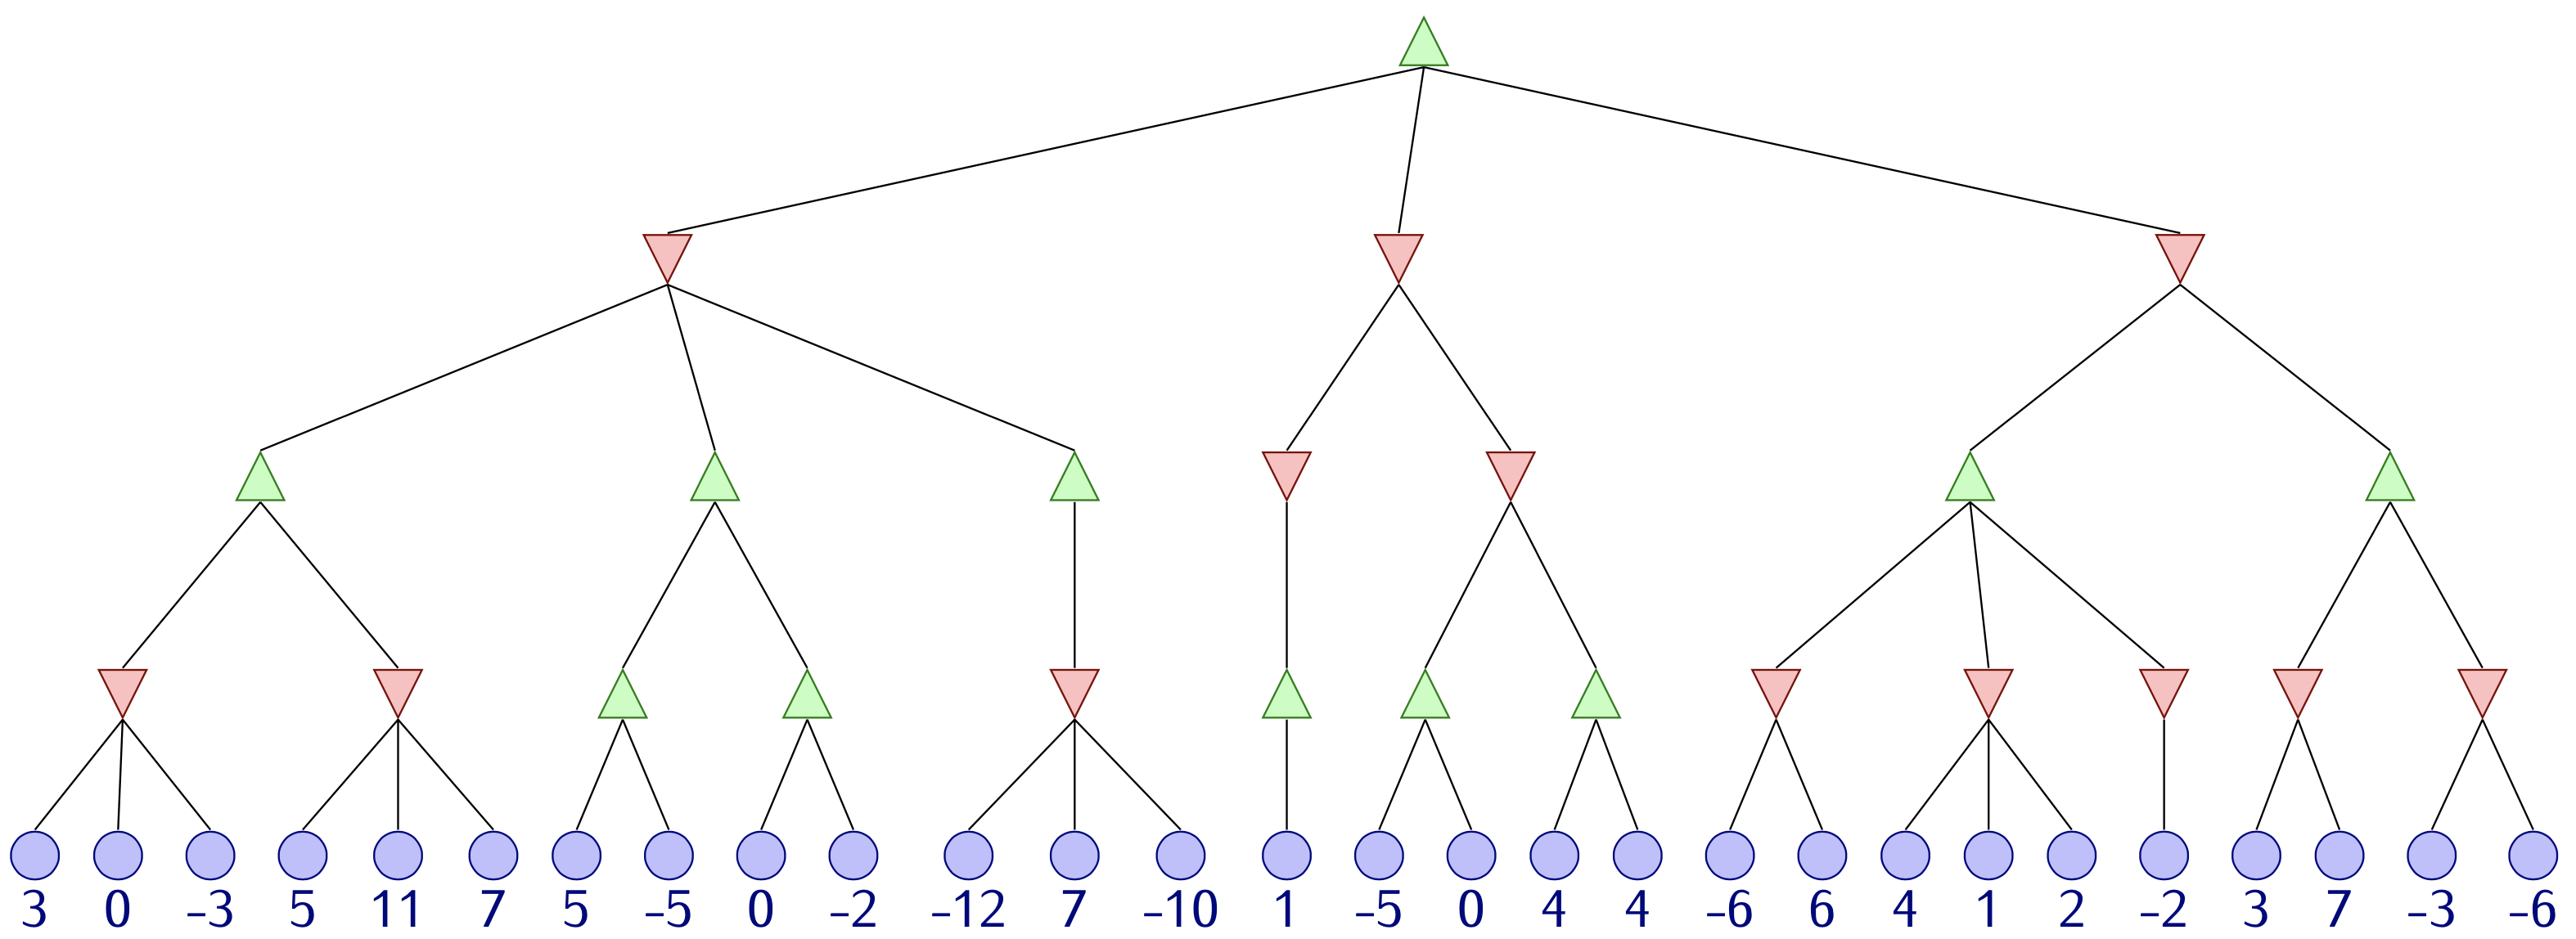
\includegraphics[scale=.29]{images/minimax.png}
\end{answers}




\begin{enumerate}
\item[5.] How does Alpha-Beta need to be modified for games with more than two players? \textbf{(1~pt)}
\end{enumerate}

\begin{answers}[9cm]
If you wish to implement Alpha-Beta for games that allow more than two players, you'd need to change the way the three is made and how the different choices are made. 

Firstly, in order to store the utility of a given state, instead of simply having a singular value stored, you'd need to change it to a vector. 
This vector would contain the utility of a given state for each player.

Now, you'd also need to modify how the different nodes choose their actions. Insead of following a "classic" minmax strategy, each player now has to take the most valuable action for itself when comparing the corresponding utility values in the vectors

So in other words, you'd need to modify the evaluation that the algorithm does (and the utility as well) followed by a generalisation of the search function to work with multiple players since it is no longer a "min -> max -> min" situation but rather a "min(p1) -> min(p2) -> max(p3)".
\end{answers}





\clearpage
\section{Shobu (35~pts)}
\medskip

\subsection{Alpha-Beta agent (4 points, to be submitted on Inginious)}
\medskip


\subsection{Monte-Carlo Tree Search agent (5 points, to be submitted on Inginious)}
\medskip


\subsection{Warm-up questions (3 points)}
\begin{enumerate}
\item[1.] What is the branching factor at the start of the game? What is the mean empirical branching factor? (The branching factor is considered here as the number of possible moves that a player can do from a given state). \textbf{(1 point)}
\end{enumerate}

\begin{answers}[5cm]
    % TODO empirical branching factor ???? to check what the f it is 
    First off, we would like to mention that even with the given additionnal info above on what the branching factor is, there's still some nuance that could be clarified. 
    As specified, the branching factor is the number of possible moves a player can make and in this case at the beggining of the game. Depending on what we consider a "move" the branching factor will be different.

    That said, we considered a move to be counted whenever one piece moves, which means that a passive and active move combo will count as 2 moves. We analysed the sarting board and saw that the player can make 18 different moves on the light board which can result in the same move on either of the 2 dark boards, hence 18*3 but the same goes if the player choses a passive move on the dark side, so
    we end up at 18*6 = 108 for the branching factor. As for the empirical branching factor, through testing we found that it was closer to 130 to 150 with spikes over 200 when the game was playing.
    \end{answers}



\begin{enumerate}
\item[2.] What would be one (of the many) drawbacks of the simple heuristic that is imposed for the basic alpha-beta agent above? \textbf{(1 point)}
\end{enumerate}

\begin{answers}[10cm]
    % TODO check + add things there 
    We observed during our time with the agent, that a few drawbacks that are notable. One of those drawbacks is the simplicity that the agent has in some situations. Let me explain.

    We observed that with the simple heuristic, the agent had a tendency to "miss" some obvious moves to make. This is probably due to the algorithm having found a "better" state following the move it took. 
    
    Another side effect of this, is the agent, whenever playing against himself, tends to find itself in a loop of the same moves over and over again. The heuristic, being "too simple" does not incorporate the detection of such loops and the main algorithm does not either. 

\end{answers}



\begin{enumerate}
\item[3.] Considering the Monte-Carlo Tree Search algorithm, what is the hypothesis supporting the use of random simulation to estimate the win rate? Is this hypothesis always valid? \textbf{(1 point)}
\end{enumerate}

\begin{answers}[15cm]
    % TODO put your answer here
    The hypothesis supporting the use of random simulations to estimate the win rate is that, even if the individual actions are random and unrealistic / suboptimal,
    their aggregated results will provide statistical information about different moves in a given state. 
 
    As for the question of validity in all cases, it is not. While it may often provide some solid foundation, there are scenarios where it does not apply due to 
    the specific nature of the game / problem the agent is trying to solve. 
    
    Here are some cases where the Monte Carlo Hypothesis may not hold:
    
    Complexity of the Game too high: In games or decision-making problems with extremely high branching factors or complex state spaces, the Monte Carlo Hypothesis will not hold. The amount of possible outcomes and interactions will make it complicated to obtain accurate estimates through random sampling alone.
    In those cases it is better to not use completely random simulations but rather make a more educated guess on which move might be fruitful.

    Depth necessity: There are some games that require deep thinking and planning in order to make the "optimal" move. 
    In those games, relying on purely random simulations may not reflect the nuances and strategies used for optimal gameplay. 
    In other words, players may employ sophisticated strategies that are not reflected in the results of random simulations, leading to inaccurate win rate estimates.

    There are other cases in which this hypothesis might not be the best choice, however those explained above are the most
    suited for the context of the game Shobu.
\end{answers}


\newpage
\subsection{Description of your agent (8 points)}
Describe in the boxes below what you have implemented for your contest agent. You can also mention things that you tried and did not work but focus on what you have submitted in the end.

\begin{answers}[21cm]
    % TODO explain your agent here
    When we first started pondering about how to approach the problem with our agent, we thought about the two different algorithms 
    we did before as a possible starting point. This lead us to consider both pros and cons for each of them and how we could improve them.
    Eventually, we decided to go with the Alpha-Beta algorithm as it was the one that gave us the best results from the get go
    while also being the one that we saw the most potential for improvement. 
    
    Speaking of improvements, the first thing we wanted to change was the heuristic. As explained before, the heuristic
    used in the basic Alpha-Beta agent was too simple and did not take into account some important aspects of the game. 
    Our new heuristic now takes into account multiple factors such as the need to defend, or the possibility of taking down
    an opponent's piece. Whilst not completely solving the issue of the agent getting stuck in loops if played against itself,
    this, along with the increase of the maximum depth allowed, proved to be more efficient than the previous case.
    To be clear, this heuristic is not by no means perfect, it's just the one that we found to be the most efficient through
    sheer trial and error.

    With this done, we tried to solve the looping issue. Our approach for this was a simple one, if we let the agent do more 
    moves in its simulations, aka, further increase the depth of the search, it would naturally detect that the actions that lead to 
    the loop are less optimal that the other choices and by such, not select them. With this, we realised that we would need to 
    increase the performance of the agent itself, since simply increasing the depth would make the agent run so slow that it would
    just timeout. 

    The first idea to improve the performance was to implement a way for the agent to not simulate states it had already seen before. 
    We did this by implementing a dictionnary where we stored the different states and the corresponding utility values for them, 
    this way, if the agent found itself in a state it had already seen, it would just take the utility value from the dictionnary and
    call it a day. This helped us reduce the occurences of loops quite a bit !

    That said, even if this sped up the agent in a non negligible way, we still needed to improve it further. This prompted us to 
    implement a way to sort the different actions the agent could take in a way that would try to maximise the preformance 
    by allowing the agent to cut off the search earlier (see the exmaples above, in question 1). 
    This allowed the agent to also be more efficient in its search and made the response time of the agent better. 

    Next, to completely solve the looping issue, we implemented a more direct way to detect if the agent was in a loop by using the 
    stored information in the dictionnary. If the agent knows that a given set of actions will lead to loop on one he did before,
    it will simply ignore those actions and try to find a better one. 

    Lastly, we still wanted to improve the performance of the agent even further. We did this by implementing a bitmap. 
    We did consider a boolean map, however we found that the potential advantages of a bitmap outweighed the complexity
    this task would bring. 

    Our bitmap was used to store the whole game state, this included the representation of the different boards and the 
    different actions to take. We also made the choice to switch our dictionnary to store elements in the form in which
    they appeared in the bitmap. How did they appear in the bitmap? Well, firstly we stored the different boards 
    as a uint16 value. This allowed us to set bits, that are in the same position as the different pieces on the board, to 1 hence resulting 
    in a uint16 value (4 rows of 4 bits each).  
\end{answers}

\begin{answers}[23cm]
    % TODO continue your answer here
    To differentiate which player's pieces were reprensented in a given uint16 value, we used a mask, thus having a simple 
    index to know which player's pieces were where. With this representation, we could easily update the dictionnary. 
    What we did, was create a string that concatenated the different uint16 values of the different boards and used this as the 
    keys for the dictionnary. This essentially allowed us to have a unique key for each representation of the game without 
    having to hash the entire state of the game. 
    To those keys we associated an array containing the binary board, the player id (which player is playing at that point),
    another array containing the keys to direct children of this state following actions taken, the utility at this state
    as well as the max and min depth this state can reach. 
\end{answers}

\begin{answers}[23cm]
    % TODO continue your answer here
\end{answers}



\newpage
\subsection{Comparison of agents (5 points)}
Describe here the comparison of the different agents: random, Alpha-Beta, MCTS and your agent (and others if you want!). Remember that it should be a statistical comparison. Describe how you compare the agents. Draw some observations and conclusions based on the results you have obtained.

\begin{answers}[20cm]
    % TODO explain your comparison method and draw conclusions
    We compared the different agents by making them play against each other multiple times and in different positions (starting and not starting).
    We looked at the win rate of each agent, the average number of moves it took for the game to conlcude as well as the reponse time of the agents.
    First off, about the random agent, it is as its name implies a completely random agent. It generates the different moves it can make
    and the just picks one at random. By the nature of this philosophy, the random agent is the agent that lost the most games. Well, it's not 
    suprising since it's just picking random moves, but this also means that its response time is the fastest of all agents since, well, 
    it doesn't have to think about what move to make.

    That said, now we can focus on the more intersting agents. The Alpha-Beta agent was by far the best choice for Shobu when compared to 
    "random" and a by the book version of "MCTS". It had the highest win rate, the lowest average number of moves and was on par with 
    "random" when it can to responsiveness. 
    Here are some stats, the Alpha-Beta agent won 100\% of the games it played against the random agent (shown in the graph below) and it averaged 
    33.60 moves per game when playing white and 16.40 moves per game when playing black. As the time it took to play the games we have an averge of 3.1s per game.
    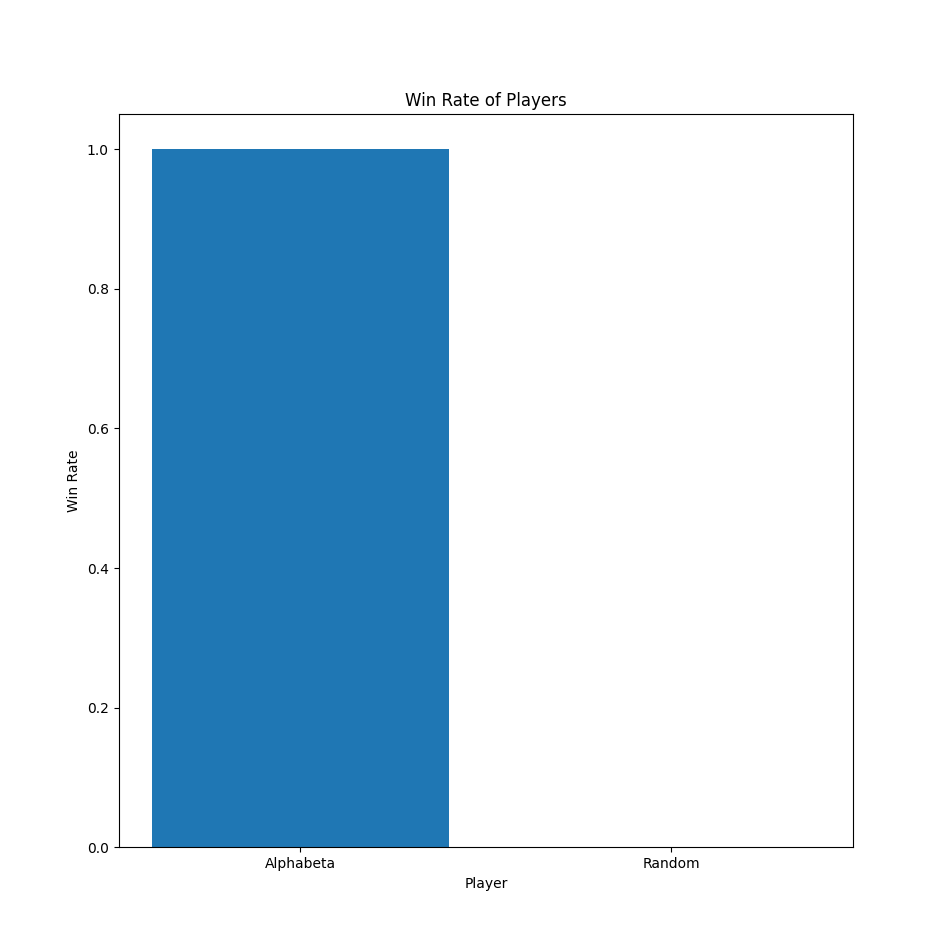
\includegraphics[scale=.29]{graphs/abvsrand.png}
    Compared to the MCTS agent, the Alpha-Beta agent was also the best choice. The Alpha-Beta agent had a win rate of 0\% against the MCTS agent and an average of
    33.60 moves per game when playing white and 16.40 moves per game when playing black. The time it took to play the games was 3.1s per game. In other words the basic 
    version of Alpha-beta is the best choice we have when in comes to agents other than ours.

    The second best was the MCTS agent. It had a hard time against Alpha-Beta, but it also did not waver against the random agent. That said it was the slowest of all agents by a margin. 
    Unfortunately, this comes from the nature of the algorithm itself. It does way too much simulations and this is reflected in the time it takes to play a game. 
\end{answers}

\begin{answers}[23cm]
    % TODO continue your answer here
\end{answers}

\begin{answers}[23cm]
    % TODO continue your answer here
\end{answers}


\subsection{Contest (10 points, to be submitted on Inginious)}



\end{document}
